\chapter{DMD applied to the IL-10-GAG system}

The previous chapter presented Dynamic Molecular Docking (DMD), a novel
molecular dynamics-based local docking method well-suited for exploring
protein-GAG interaction. I applied DMD to the IL-10-GAG system, using the
binding region prediction derived in \cref{chapter:bspred}. The goal was to
further characterize the interaction of GAGs with IL-10 in that region, and to
identify potential molecular mechanisms of IL-10-GAG interaction. This chapter
seeks to present \textit{i)} the computational challenges, \textit{ii)} the
methodological details, and \textit{iii)} the major outcomes of this endeavor.

Several DMD studies were performed, with varying DMD parameterization as well as
varying molecular system setup. Conducting these studies required an increment
of the computational resources available to us by orders of magnitude. In the
course of performing these studies I continuously refined the software
architecture for controlling the corresponding high performance computing
resources and enriched the DMD data analysis framework, as described in this
chapter. One of the main results of the IL-10-GAG DMD studies presented here is
the identification of IL-10's R107 as key residue for GAG binding.


\section{Methods}

\subsection{Overall study design}
\label{dmdil10:overallmethod}

As a reminder, the term DMD study covers many DMD run repetitions followed by
data analysis. Hence, within a single DMD study the \textit{constants} are ---
among others --- the chemical configuration of the ligand molecule and the
geometrical DMD parametrization, i.e.\ the protein core atom and the focus
point. Clearly, a systematic investigation of the IL-10-GAG system via DMD
requires \textit{variation} of exactly these entities. Consequently, the planned
investigation requires the conduction of \textit{many} DMD studies. Initially,
the conduction and analysis of a single study consumed about two weeks. That is,
time and computational resources were the main limiters of the extent of this
endeavor. Hence, the goal was to get as much conclusive output out of as few DMD
studies as possible.

\subsubsection{Factors to investigate}

The entities that are obviously interesting to vary among the different DMD
studies in case of the IL-10-GAG system are:

\begin{itemize}

\item[1)] \textbf{The DMD protocol.} In the course of performing various DMD
studies I aimed for slight protocol changes for optimizing the computational
efficiency of DMD, compared to the protocol initially developed for the DMD
validation study described in \cref{chapter:dmd}. We decided to potentially
optimize parameters such as decreasing the tMD simulation length as well as the
LROM displacement length, both of which have direct impact on the pulling
process velocity. A the same time, I tried to increase the number of
independent DMD run repetitions within single DMD studies as far as our
computational resources allowed to, in order to obtain as much sampling
performance as possible.

\item[2)] \textbf{The geometrical DMD parameterization.} In
\cref{chapter:bspred}, a putative IL-10-GAG binding region was derived, which
can directly be used as input for designing IL-10-GAG DMD studies. For
potentially discovering a distinct and well-defined binding \textit{site} and
for investigating and finally eliminating the impact of the geometrical DMD
parameterization on any conclusion about the IL-10-GAG system, I decided to vary
DMD focus point and entry lane among the DMD studies. One should note however,
that in order to obtain reliable information about the impact of other
variables, this one here should stay constant most of the time, which is why I
decided to try only two different geometrical setups in a first stage of DMD
studies, and a final third geometrical parameterization in a second stage of
DMD studies. The terms \textit{first stage} and \textit{second stage} will be
used throughout the upcoming sections of this chapter.

\item[3)] \textbf{The representation of IL-10's N-terminus in MD simulations}.
In IL-10's crystal structure with PDB ID 2ILK the first 5 residues of the
N-terminus are not resolved as of their flexibility. This N-terminus is
spatially close to the putative GAG binding region derived in
\cref{chapter:bspred}. This is an unfortunate situation, because if this
terminus plays a role in GAG recognition, it would not easily be possible for us
to detect it --- modeling the behavior of such a flexible / disordered terminus
is not possible with all certainty and requires special sampling techniques on
its own, not \textit{per se} combinable with DMD. However, the N-terminus is
expected to be less important for specific GAG interaction than the amino acid
residues in the region identified and since simulating the disordered N-terminus
without special treatment is pointless, these five residues were omitted from
most of the MD simulations. In addition, for having a comparison, and for
obtaining an idea about its possible impact, I decided to include the
N-terminus in at least one or two test case DMD studies.

%, as of the strong electrostatic attraction towards that
%\textit{static} region, and the  expect take the flexibility and sequence as an argument that


\item[4)] \textbf{The chemical configuration of GAG ligands.} For identifying
characteristic differences among different GAG types and lengths with respect to
their interaction with IL-10 it was required to perform DMD studies with
constant conditions while varying the chemical configuration of the GAG
molecule. A decision was taken about which GAG types/lengths are most
interesting for investigation, resulting in the following selection of GAG
molecules:

\begin{itemize}

\item \textit{Heparin} (HP), a must-have in this list, as its interaction with
IL-10 has been experimentally confirmed previously \cite{salek_ardakani_2000}. I
decided to investigate heparin tetra- as well as hexasaccharides: in the DMD
validation study it was shown that DMD is capable of properly sampling the
internal degrees of freedom of GAG hexasaccharides. For longer GAGs, however, it
would be uncertain whether the sampling is sufficient and, with that, the
reliability of the results. Investigating tetrasaccharides in addition to
hexasaccharides is useful for observing potential (in)consistencies in the
observations depending on GAG length. Disaccharide investigation, however, would
likely be a waste of computational resources, since protein-GAG binding
specificity can usually not be established for such short GAGs (the vast
majority of GAGs in protein-GAG complexes in the PDB hast more than two sugar
rings only).

\item \textit{Hyaluronan} (HA), which is the only natural GAG free of sulfation.
As of its lack of sulfate groups, besides of being less charged, it has
significantly different spatial properties than e.g.\ heparin: it is less bulky.

\item \textit{Chondroitin-4-sulfate} (CS4) and \textit{Chondroitin-6-sulfate}
(CS6). The chondroitin sulfates are important representatives of the class of
GAGs. Compared to heparin, the 4- and 6- variants of chondroitin sulfate have
two sulfate groups less per disaccharide unit (only one) and are therefore less
charged and less bulky. In CS6, carbon 6 of the N-Acetyl\-ga\-lacto\-sa\-mine is
sulfated, meaning that the sulfate group is protruding further into space than
in case of CS4, where the sulfate is attached directly to the ring (cf.
\cref{intro:gags}), providing this GAG with quite different spatial properties
than CS4.

\end{itemize}

\end{itemize}

\subsubsection{Iterative approach}

For the global design of our DMD studies, I decided to take an iterative
approach. In a first stage, I aimed to gather experience about how the IL-10-GAG
system responds to various kinds of DMD parameter changes. Furthermore, since
the technical environment was unstable, I used this first stage of studies for
detecting and resolving technical issues. Hence, in this first stage of studies,
I varied the conditions according to all points described above, with the goal
to obtain stable conditions applicable in a second stage, together with an
optimized geometrical DMD parameterization.


\subsubsection{Automated DMD data analysis}

For efficiently breaking the enormous amount of raw data produced by any DMD
study down to human-interpretable essentials, we specified and implemented an
automated data analysis framework. In this framework, every DMD run within a DMD
study is assigned a unique identifier. Subsequently, we extracted all
\textit{static} and \textit{dynamic} quantities for each DMD run listed in
\cref{dmd:dataanalysis}, and assigned those quantities to the corresponding
run identifiers. As a result, we obtained a table of dimensions $N \times M$,
with $N$ being the number of DMD runs and $M$ being the number of
single-run-derivable quantities. In a second class of analyses, the
ensemble-derivable quantities as described in \cref{dmd:dataanalysis} were
extracted from all runs in the DMD study, usually based on the single-run data
extraction performed before. Finally, we clustered the docking solution ensemble
using the method described in
\cref{chapter:bspred}.

The resulting reduced set of data allows for a broad subsequent data analysis.
For instance, any two single-run-derivable quantities can easily be correlated
for understanding their relationship, or the distribution of any extracted
quantity can easily be looked at and statistically evaluated. Furthermore, our
data analysis framework allows for generating cluster statistics based on the
\textit{clustering} of docking solutions. For instance, the average ligand
mobility within a certain cluster is easy to obtain. This enables meaningful
comparison of clusters by those properties, especially among \textit{different}
DMD studies.


\subsection{Computational framework}


\subsubsection{High performance computing requirements of one DMD study}

One DMD study according to the protocol as presented in \cref{chapter:dmd},
i.e.\ with $N = 100$ repetitions, a pulling process simulation time of
\SI{4}{\nano\second} and a free MD simulation time of \SI{10}{\nano\second}
implicates about \SI{1.4}{\micro\second} of simulated real time. As of these
numbers, one DMD study requires about 12 years ($10^5$ hours) of accumulated CPU
time using state-of-the-art hardware (such as the Intel Xeon Processor X5650).

In high performance computing (HPC), computational tasks are usually abstracted as
\enquote{jobs}, whereas a job is a sub-problem of an \enquote{embarrassingly
parallel} problem \cite{heath1986hypercube}, for which little or no effort is
required to separate the problem into a number of independent tasks. For
efficient use of HPC batch schedulers for DMD, we have abstracted a DMD study
into the following list of jobs (whereas some of the jobs named later in the
list require completion of those listed earlier):

\begin{itemize}
\item LROM system preparation jobs (minimization, heat-up, equilibration)
\item $N$ tMD production jobs
\item $N$ free MD jobs (minimization, heat-up, equilibration, production)
\item $N$ final state validation and energy minimization jobs
\item $N$ free MD trajectory analysis jobs (MM-PBSA)
\item $N$ free MD trajectory analysis jobs (MM-GBSA + SRED)
\item $N$ free MD trajectory analysis jobs (geometry and hydrogen bonding
analysis)
\end{itemize}

Depending on $N$, this yields on the order of $10^3$ computing jobs per DMD
study. The raw data created by those jobs comprises on the order of $10^2$
gigabytes distributed in about $10^5$ files.


\subsubsection{Establishment of GPU computing resources}

Initially, the execution of a single DMD study was possible for us within about
three weeks, using the \enquote{Atlas} resource pool in the supercomputing
center of the TU Dresden (ZIH), which provisions a large number of AMD Opteron
6274 CPUs. However, this system was affected by many technical issues, ran out
of support by the ZIH, and did not reliably allow us to perform various DMD
studies in parallel, or even increase the number of DMD run repetitions $N$. The
in-house computing cluster of the BIOTEC, TU Dresden (the
\enquote{biocluster}, comprised of about 30 machines) was out of question for
performing DMD studies as of too few resources.

For mitigating issues related to a lack of computing resources for DMD, we were
early adopters of a new technology: the usage of graphics processing units
(GPUs) for general purpose computing (\enquote{GPGPU} \cite{wikipedia_gpgpu}).
Simply spoken, GPUs make heavy use of the so-called single instruction, multiple
data paradigm (SIMD, see \cite{kirk2012programming_gpus} for further
information), which matches common algorithms used in MD simulations very well.
That is, MD simulations can take strong advantage of GPU architectures. Compared
to classical computing architectures, this leads to \textit{i)} a significantly
higher absolute simulation performance (measured in nanoseconds of simulated
time per day) and \textit{ii)} a much better performance per financial cost
ratio, considering acquisition cost as well as energy cost. With the MD
simulation framework Amber 12 \cite{case_amber_12} and corresponding patches
\cite{amber_12_patches}, the Amber developers were among the first to work on
and release a solid and efficient MD implementation for GPUs (pmemd.cuda, see
\cite{amber_gpu_2012,amber_gpu_pme_2013} for methodological details and
validation).

Correspondingly, we engineered a GPU computing cluster in our research group,
which required substantial amounts of planning and testing, because no
enterprise-level vendors were available for this kind of hardware. Hence, we
composed this cluster based on raw hardware and software components, eventually
yielding the following configuration:

\begin{itemize}
\item Four dedicated compute nodes, based on low-clocked Intel central
processing units on special consumer-level mainboards, placed in
temperature-regulated server racks.
\item A total of 15 GPU devices distributed among these machines (2 Tesla C2070,
3 GTX 580, 2 GTX 690, 4 GTX 770, 4 GTX TITAN, all Nvidia CUDA devices
\cite{nvidia_cuda_devices}, purchased in batches spread across 1.5 years).
\item Linux operating systems, along with appropriate drivers and CUDA runtime
libraries.
\item A customized Torque \cite{torque_website} GPU job scheduling system, see
\cite{gehrcke_torque_gpu_setup} for details.
%\item pmemd.cuda, built
\end{itemize}

With this infrastructure at hand, we were able to perform a single DMD study
within less than two weeks, without being dependent on \textit{external}
resources. On top of that, from summer 2013 on we have been part of the testing
period of the large-scale GPU computing cluster of the supercomputing center of
the TU Dresden: as a section of their \enquote{Taurus} platform, they provide 80
Nvidia CUDA GPU devices. All in all, with these GPU resources at hand, we were
able to perform single DMD studies on a weekly basis, with a significantly
increased number of DMD runs per study ($N=200$ or $300$). \hl{In Dresden, this
would not have been possible using classical computing resources. keep this?}.


\subsubsection{Software architecture}

Above, we derived that one DMD study is comprised of on the order of $10^3$
computing jobs, and that it requires storing hundreds of gigabytes of raw data
distributed in about $10^5$ files. These numbers suggest that the management of
corresponding jobs and data requires a well-engineered DMD controlling system.
The essential purpose of such system is to automatically identify errors and
recover from those: the likelihood for a single computing machine to fail times
the number of machines involved in a DMD study integrated over the computing
time yields a significant probability for the study to be affected by
\textit{one or more} technical issues. In other words, there is a guarantee
that something will go wrong. By experience we can tell that this prediction
came true, and manual identification of corresponding issues was a daunting
task, which is why we iteratively developed a system architecture that enables
the efficient conduction of DMD studies.

One requirement for this management architecture was to support all involved
hardware platforms, i.e.\ the Taurus GPUs, the Taurus CPUs (for data analysis),
the group-internal GPU cluster, and the biocluster CPUs (for data analysis),
whereas these platforms alone involve three different batch scheduling systems.
As all of these platforms are based on POSIX-compliant operating systems with
reliable and well-performing file systems attached, we abstracted the data
structure for managing and monitoring a DMD study on top of the file system
hierarchy, and implemented basic data creation, manipulation, and validation
using well-established POSIX command line tools, incorporated in shell scripts.

For many purposes of data validation and analysis we implemented Python
programs based on Biopython \cite{biopython_web} and SciPy/NumPy
\cite{scipy_numpy} whenever appropriate. Data plotting was performed using
the Python module Matplotlib \cite{matplotlib_web}. Iterative development and
continuous integration of this software architecture was largely facilitated by
the efficient usage of a decentralized version control system (Mercurial
\cite{mercurial_web} in this case). For reference, the corresponding code
repository is available at \url{http://bit.ly/jgehrcke-phd-dmd-control}.


\subsection{Geometrical DMD parameterization}
\label{dmdil10:method_geom_setup}

\begin{figure}
\centering
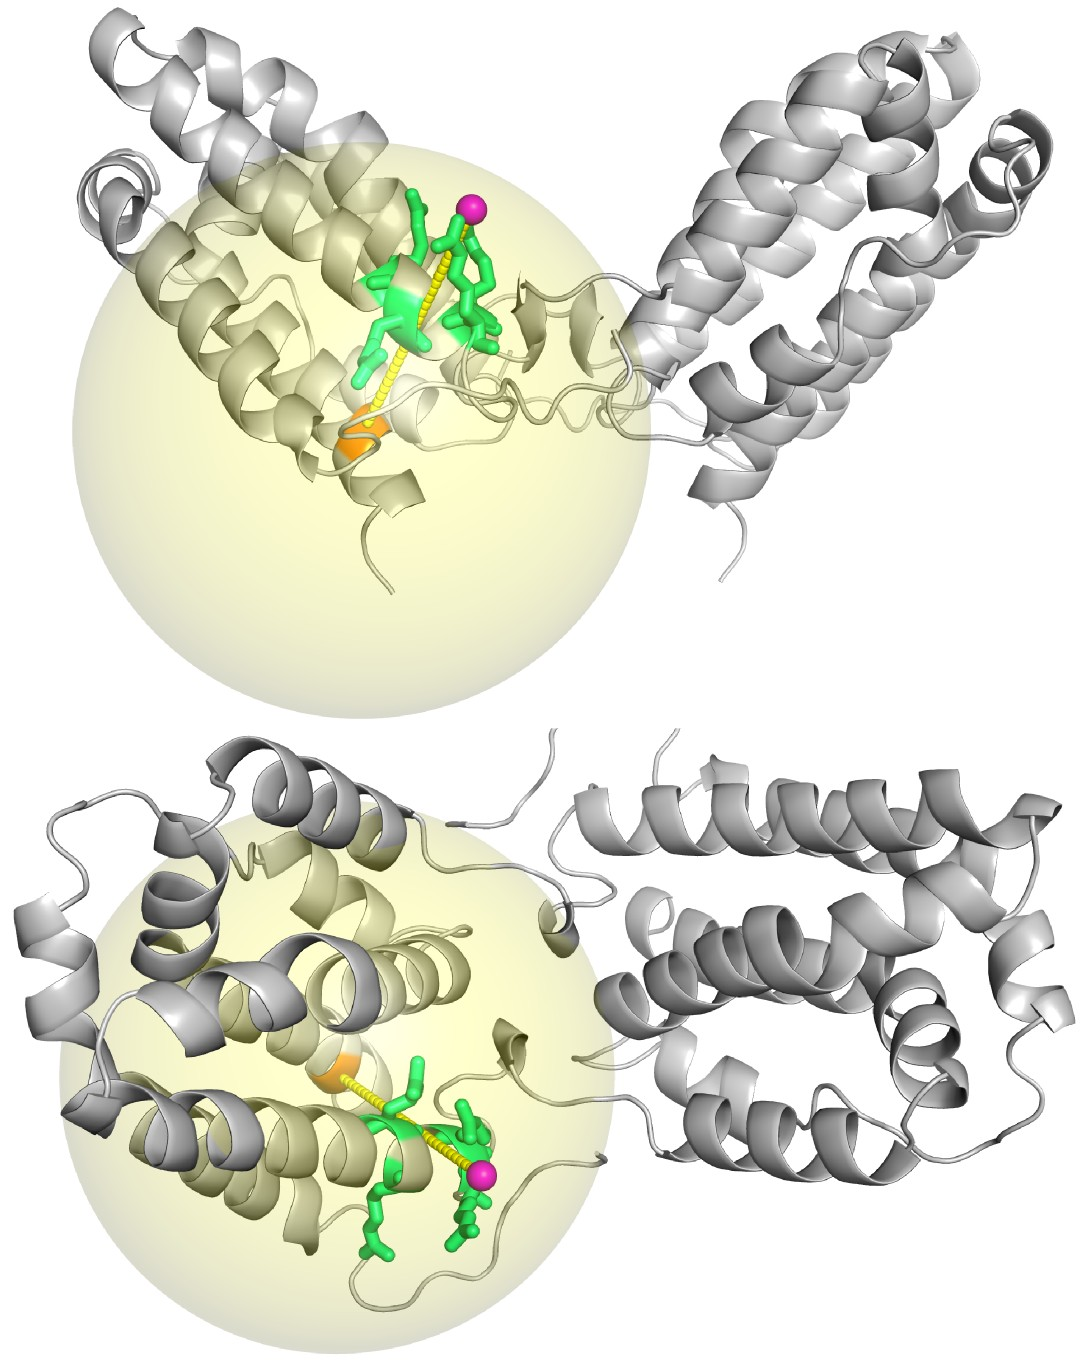
\includegraphics[width=1.0\textwidth]{gfx/dmdil10/round1_il10_ligandcenter_proteincore_sphere_top_and_side_001.jpg}
\caption[]{Geometrical DMD parameterization used for most of the DMD studies
in the first stage. The IL-10 dimer is shown in gray ribbon representation (top:
side view on the V-shape, bottom: top-down view on the V-shape). The C-alpha
atom of methionine 154 in the human interleukin-10 sequence was selected as
protein core atom (ribbon colored in orange). The focus point (small sphere
colored in magenta) was selected manually based on the putative binding region
comprised by residues R102, R104, R106, R107 (colored in green sticks). The tMD
target distance of \SI{17.7}{\angstrom} between the protein core atom and the
focus point is indicated by a thick yellow dashed line. The large transparent
yellow sphere is centered on the protein core atom and its radius is set to the
tMD target distance. It visualizes the surface that contains all central ligand
atoms after tMD.}
\label{fig:dmdil10:dmd_geometry_round1}
\end{figure}

\Cref{fig:dmdil10:dmd_geometry_round1} visualizes the geometrical DMD
parameterization used for most of the DMD studies in the first stage. The manual
selection of core atom and focus point was based on the binding site prediction
made in \cref{bspred:il10} and performed in compliance with the guidelines
formulated in \cref{dmd:lrom_preparation}. We ended up using the C-alpha atom of
M154 as core atom, and a tMD target distance of \SI{17.7}{\angstrom}, yielding a
quite large spherical surface for proper putative binding site sampling. If
relevant, deviations from this geometrical setup in the first or second stage of
DMD studies are described in the results and discussions part.


\section{Results and discussion}

\subsection{1st stage of DMD studies}

\subsubsection{DMD result consistency}

One of the first results in this stage of IL-10-GAG DMD studies was the
observation of method consistency, i.e.\ support for sufficient sampling and
convergence of the DMD method.
\Cref{fig:dmdil10:hp_hexa_vs_tetra_clusters_position_match} shows the overlay
of two clustering results from two independently performed DMD studies that
differed \textit{only} in the GAG ligand length --- one was performed with a
heparin hexasaccharide, and the other with a heparin tetrasaccharide.
Rationally, one would require DMD to return a very similar binding pose
prediction in both cases, as it is unlikely for these GAG types to behave
fundamentally different. As motivated in \cref{relevance_of_clustering},
comparison of the position of the most populated clusters in both cases is a way
to (in)validate this assumption. Note that comparison of both clusters, and with
that, comparison of both DMD studies with respect to the distribution of docking
solutions, is only possible because we took great care of making both clustering
results comparable via the clustering parameter optimization described in
\cref{clustering_param_opt}. In both cases, the docking solution clustering was
performed with $N_{min}$ (the minimal number of clusters that must be found) set
to 1, and $M_{min}$ (the minimal number of members within each cluster) set to
4. In both cases, the automatic clustering parameter optimization yielded an
   $\epsilon$ value of \SI{2.6}{\angstrom}, i.e.\ just about the same density of
   docking solutions in both clusters.

\begin{figure}
\centering
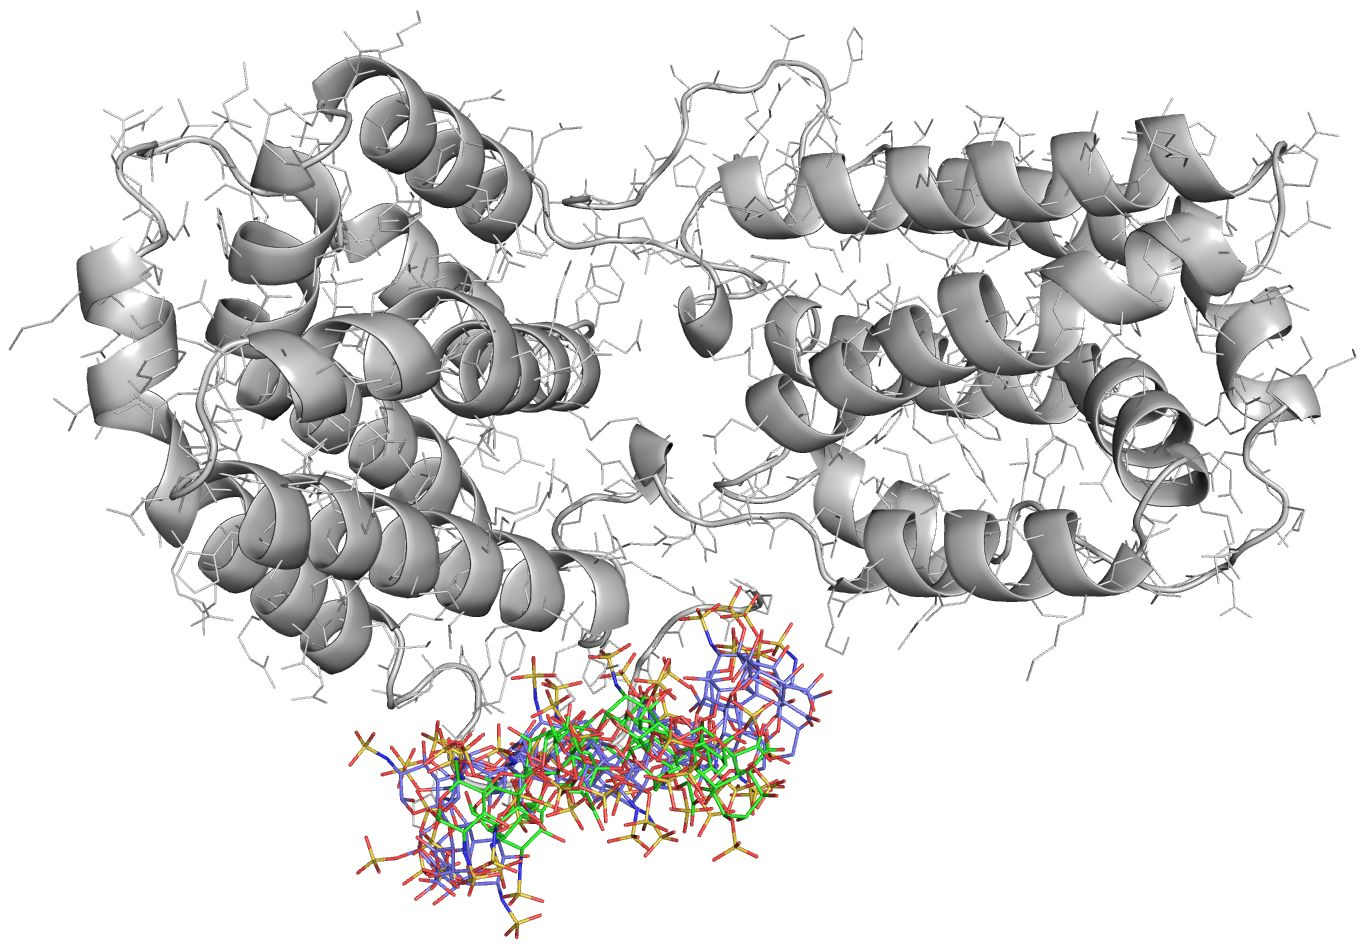
\includegraphics[width=1.0\textwidth]{gfx/dmdil10/hp_hexa_vs_tetra_clusters_position_match_cropped.jpg}
\caption[]{Consistent results among two independently conducted DMD studies. The
IL-10 structure is shown in gray cartoon/line representation. The most populated
cluster of docking solutions derived from a DMD study with a heparin
hexasaccharide is shown with carbon atoms in blue. The most populated cluster of
a corresponding DMD study with a heparin tetrasaccharide is shown with carbon
atoms in green. Setup and protocol of both DMD studies differed \textit{only} in
the GAG ligand length.}
\label{fig:dmdil10:hp_hexa_vs_tetra_clusters_position_match}
\end{figure}

In essence, both clusters are positioned equivalently with respect to IL-10, and
show the same density. That is, with respect to the distribution of docking
solutions, both DMD studies returned the same result. In addition to the DMD
validation study presented in \cref{chapter:dmd}, this result supports the
significance of data created by the DMD method.


\subsubsection{Impact of N-terminal residues and modest geometry changes}
%NOTE: when changing this heading, also change the "quote" in the section
% \subsubsection{Ensemble-derived single-residue energy decomposition} below.

In one of the early studies we included the five N-terminal residues of IL-10
(see \ref{dmdil10:overallmethod}) and varied the geometrical parameterization of
DMD compared to the setup described in \ref{dmdil10:method_geom_setup}: we kept
the C-alpha of M154 as core atom, but slightly changed the focus point within
the anticipated binding region, resulting in a different orientation of the
yellow axis shown in \cref{fig:dmdil10:dmd_geometry_round1}, and in a tMD target
distance of \SI{20.5}{\angstrom}. The rest of the system and protocol setup was
equivalent to another DMD study with a heparin tetrasaccharide, whose
geometrical outcome is shown in
\cref{fig:dmdil10:hp_hexa_vs_tetra_clusters_position_match}. As it turned out,
the final distribution of docking solutions was not affected by both changes, as
the most populated cluster matched the position of the clusters shown in
\cref{fig:dmdil10:hp_hexa_vs_tetra_clusters_position_match}.

We conclude that the results of a DMD study are rather insensitive with respect
to modest changes in the geometrical parameterization of DMD, and that the
presence of the five N-terminal residues does not significantly affect the DMD
binding pose prediction, and therefore is not of the highest priority to study.


\subsubsection{Distinction among GAG types by single-run quantity cluster stats}

\begin{table}
\footnotesize
\centering
\renewcommand{\arraystretch}{1.3}
\begin{tabular}{lcrll}
\midrule
GAG type                 & cluster members & $\epsilon$ (\si{\angstrom}) & $m$ (\si{\angstrom}) & $\Delta G$ (\si{\kilo\calory\per\mol}) \\
\midrule
HP dp6                   & 4               & 2.5                         & 2.8 $\pm$ 0.7          & -45 $\pm$ 15                           \\
CS4 dp6                  & 5               & 3.2                         & 2.6 $\pm$ 0.3          & -37 $\pm$ 8                            \\
CS4 dp6 (2nd cluster) & 4               & 3.2                         & 2.4 $\pm$ 0.4          & -37 $\pm$ 14                          \\
\midrule
\end{tabular}
\caption{
Characterization of most populated clusters by single-run quantity cluster stats
for two different DMD studies differing \textit{only} in the GAG type. In one
study, we used a heparin hexasaccharide (dp6), in the other we used a
chondroitin-4-sulfate (CS4) hexasaccharide. The heparin study yielded a single
prominent cluster, the CS4 study yielded two similar clusters. $\epsilon$ is the
spatial density of docking solutions according to \cref{clustering_param_opt}.
$m$ is the mobility of the ligand relative to the receptor, as defined in
\cref{dmd:dataanalysis}. Here, $\Delta G$ is the free energy of binding
estimate as provided by the MM-PBSA method \cref{methods:mmpbsa_mmgbsa}. The
standard deviations shown are derived from the cluster-internal variations.}
\label{tab:dmdil10:round1_different_gag_types}
\end{table}

Ideally, different behavior of different GAG types is expressed in the docking
solution clustering, and especially in the single-run quantities evaluated on a
per-cluster basis. The characterization of most populated clusters for two
different DMD studies differing \textit{only} in the GAG type should be
discussed by means of an example. In one study, we used a heparin hexasaccharide
(dp6), in another we used a chondroitin-4-sulfate (CS4) hexasaccharide. The
heparin study yielded a single prominent cluster, the CS4 study yielded two
similar clusters. The placement of the clusters relative to IL-10 was similar
(data not shown), and the quantitative evaluation of both clusters yielded
similar results, see \cref{tab:dmdil10:round1_different_gag_types}: among the
three clusters, the ligand movement relative to the receptor as well as the
MM-PBSA free energy of binding estimate are indistinguishable, considering the
cluster-internal fluctuations represented by the standard deviations. Just the
cluster density indicates that the docking solutions obtained for heparin show a
little more spatial consistency than the solutions obtained for CS4.

The important conclusion to be drawn from this and comparable observations (data
not shown) is that the IL-10-GAG system does not easily allow for a binary
(\enquote{black-white}) distinction of different GAG types via DMD with respect
to their role for IL-10 function modulation.


\subsubsection{Ensemble-derived hydrogen bonding information}

\begin{figure}
\centering
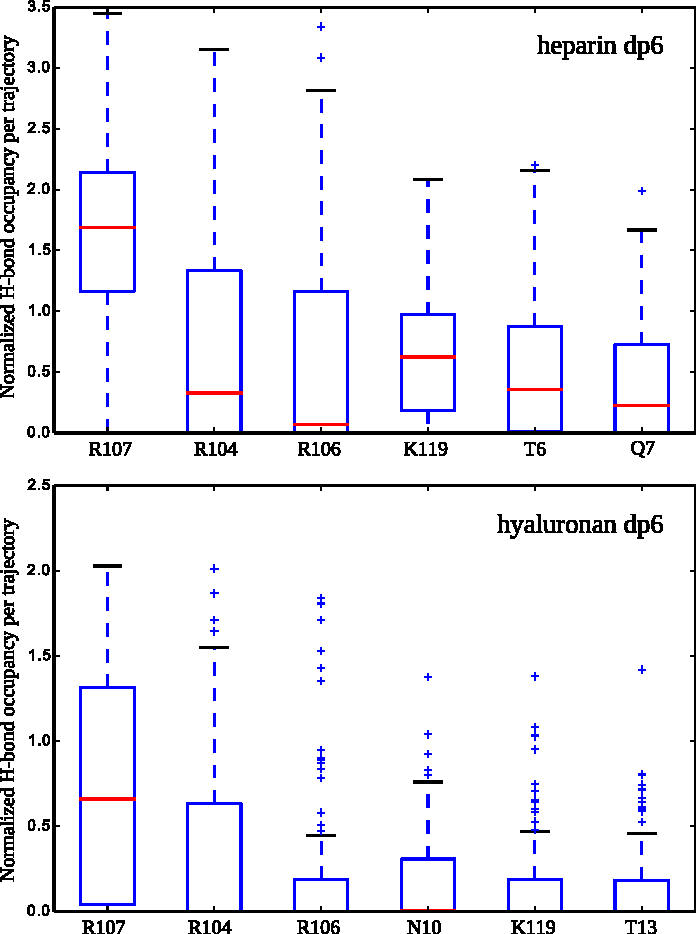
\includegraphics[width=1.0\textwidth]{gfx/dmdil10/round1_il10_hbond_hadp6_vs_hpdp6.pdf}
\caption[]{Most important residues of IL-10 for GAG-interaction, as identified
by DMD ensemble-derived hydrogen bonding information, from two independently
performed DMD studies differing \textit{only} in the GAG type (top: heparin
hexasaccharide, bottom: hyaluronan hexasaccharide). The box plot representation
is made from  $N=100$ samples per box, whereas each sample is the number of
hydrogen bond donors integrated and normalized over the data production period
of one free MD trajectory, for the residue specified in the abscissa label.
The residues are sorted by the \textit{mean} (not shown), the red bars indicate
the \textit{median}.}
\label{fig:dmdil10:hp_hexa_vs_ha_hexa_hbond}
\end{figure}


As explained in the \enquote{extraction of ensemble properties} part of
\cref{dmd:dataanalysis}, a DMD study is able to yield reliable information
about the importance of single receptor amino acids for ligand binding, via
e.g.\ hydrogen bonding (H-bond) analysis of the MD trajectory data.
Surprisingly, \textit{all} of the DMD studies performed in the first stage of
studies returned the same clear and unequivocal result --- that R107 of IL-10
plays a major role in IL-10-GAG interaction.
\Cref{fig:dmdil10:hp_hexa_vs_ha_hexa_hbond} shows ensemble-derived H-bond
information for two independently performed DMD studies differing in the GAG
type: one was performed with a heparin hexasaccharide, the other with a
hyaluronan hexasaccharide. For each free MD trajectory in these two DMD studies
we determined the normalized occupancy of H-bond donor atoms in each receptor
residue, and ranked the results by the mean normalized occupancy. We accumulated
all donors within single residues, for instance an arginine can donate up to
three hydrogens at the same time (the maximum normalized occupancy in this case
would be 3). \Cref{fig:dmdil10:hp_hexa_vs_ha_hexa_hbond} shows the top six
residues for both studies, including box plot representations of the
corresponding distributions. In both cases, R107 is ranked first by mean (not
shown) as well as median. In case of HP dp6, we measured a mean R107 occupancy
of about 1.7, i.e.\ throughout the entire DMD study this residue donated (on
average) almost \textit{two} hydrogen atoms to H-bonds. This number alone is a
strong indicator for the relevance of this residue in protein-GAG interaction.
However, the essential observation is that R107's hydrogen bonding properties
qualitatively stand out compared to all other amino acids: the H-bond occupancy
distributions of all other residues have their maximum near 0, and a decay
towards higher occupancies, yielding a median close to 0, in both cases shown
(HP dp6 and HA dp6). The occupancy distribution of R107, however, has a median
clearly far from 0 (in case of HP dp6, the distribution has its global maximum
at about 1.5). We conclude that most of the molecular surface of R107 is
solvent-exposed, and significantly more accessible for interaction with
functional groups of GAGs than the other residues.

Obviously, hyaluronan has significantly less functional groups available that
might act as H-bond acceptors than heparin. Quantitatively, this difference is
clearly reflected in the mean of the H-bond occupancy distributions, with about
1.7 for HP dp6 and about 0.7 for HA dp6 (data not shown). For all different GAG
types and lengths investigated in the first stage of IL-10-GAG DMD studies (such
as CS4 dp4, CS6 dp4, HA dp4, HP dp4, data not shown), R107 clearly stands out by
the qualitative criteria described in the paragraph above. We conclude that R107
significantly stands out compared to all other residues and supposedly plays a
particularly important role in IL-10- GAG recognition.


\subsubsection{Ensemble-derived single-residue energy decomposition}

\begin{figure}
\centering
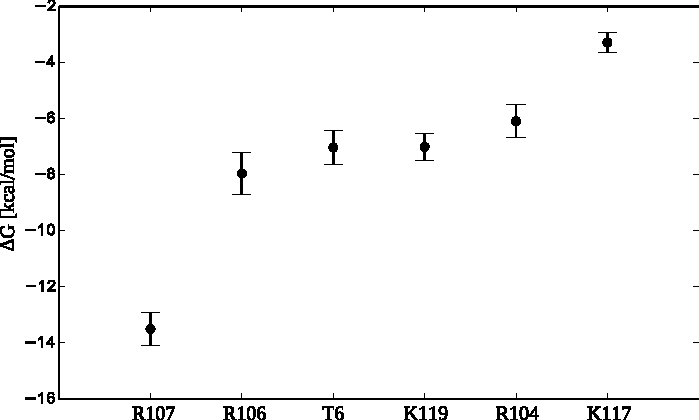
\includegraphics[width=1.0\textwidth]{gfx/dmdil10/round1_il10_SRED_hpdp6.pdf}
\caption[]{TODO}
\label{fig:dmdil10:SRED_hpdp6}
\end{figure}

We have observed the ensemble-merged MM-GBSA single-residue energy decomposition
(SRED, as explained in the \enquote{extraction of ensemble properties} part of
\cref{dmd:dataanalysis}) data to yield results generally consistent with those
of the hydrogen bonding analysis. Most importantly, the SRED data also points
out the importance of R107 for IL-10-GAG recognition.
\Cref{fig:dmdil10:SRED_hpdp6} shows the six top-ranked IL-10 residues according
to SRED performed on a DMD study with a heparin hexasaccharide. In this case,
the DMD study was comprised of $N=200$ DMD runs, and the SRED data of the top
\SI{40}{\percent} of the DMD runs according to the MM-PBSA free energy of
binding estimate has been merged, yielding about 80 DMD runs contributing to the
data shown. The error bars represent the standard error of the mean, and we can
conclude that --- considering the statistical error --- the residues on ranks
two to five are not distinguishable, ranging in the interval between
\SI{-6}{\kilo\calory\per\mol} and \SI{-8}{\kilo\calory\per\mol}. R107, however,
has a special role, with a significantly stronger mean interaction energy of
about \SI{-13.5 +- 0.5}{\kilo\calory\per\mol}. Note that the absolute values of
these energies as well as the inter-residue energy distance have no real
meaning. However, relative distances with proper consideration of the
statistical errors yield resilient information.

As in case of hydrogen bonding data, the other DMD studies with different GAG
types and lengths also revealed R107 as having the strongest interaction with
the GAG, leaving all other residues far behind (data not shown). Further
insights were derived from other IL-10-GAG DMD studies. For instance, a DMD
study with a hyaluronan hexasaccharide led to the same qualitative SRED results,
in the sense that R107 stood out. However, the corresponding mean interaction
energy was determined as \SI{-3.8 +- 0.3}{\kilo\calory\per\mol}, which is about
\SI{70}{\percent} weaker than in case of the heparin hexasaccharide study
discussed in the paragraph above. Again, qualitatively this drop is expected as
of the missing sulfate groups in HA compared to HP, and in compliance with the
hydrogen bonding data discussed in the previous section. In general, we can
conclude that both, SRED and hydrogen bonding analysis are able to identify R107
as especially important, whereas the hydrogen bonding analysis is
computationally less complex than hydrogen bonding analysis. Another interesting
observation we have made is that inclusion of IL-10's N-terminus does not
significantly influence the outcome of SRED as well as hydrogen bonding data, in
line with the conclusions drawn in the \enquote{Impact of N-terminal residues
and modest geometry changes} part above.



\subsubsection{R107A mutation}

\hl{Note (TODO):}
If there is not enough content here, do not make this a (sub)section.
Most important result: No other residue could take the role of R107.


\subsection{2nd stage of DMD studies}

\hl{Note (TODO):}
N=200 and N=300 for much clearer clustering and reduction of target displacement
length to 25 Angstroms and pulling process simulation time to 3 ns instead of 4
without observable caveats.

\hl{Note (TODO):}
Show picture of R107 specifically marked in the structure, together with
crystal sulfates, discuss possible binding poses involving these crystal
sulfates.


\subsection{Conclusions}

\hl{Note (TODO):}
So far, about 10 independent DMD studies involving IL-10 and different GAGs
have been performed. An important intermediate result of the corresponding data
analysis is that one amino acid residue, R107 (in the hIL-10 sequence, conserved
in mouse), significantly stands out compared to all other residues and
supposedly plays a particularly important role in IL-10-GAG recognition. This
conclusion is based on different types of data, including time-averaged hydrogen
bonding analysis and single-residue energy decomposition applied to MD data
collected on the microsecond time scale.

